The aerodynamic control surfaces present on the rocket were chosen to grid fins in \autoref{sec:GNC}, as used on Space X's \textit{Super Heavy Booster}. Grid fins provide longitudinal and angular control, while also giving some drag to slow down the rocket. For Space X's electric motors torque the grid fins to their desired angle, as a result a first order low-pass filter can be used to model the lag in their actuation.

\cite{washington1993grid} perform experiments on grid fins and give curves for their drag and normal force coefficients, as these are validated examples of the change in aerodynamic coefficients for grid fins these shall be used as they provide a representative benchmark. The drag coefficient is roughly equal to the axial force coefficient of the grid fins at low angles of attack, as such \autoref{fig:drag_coeff_grid} can be interpolated by using \textit{WebPlotDigitiser} to extract points on the curve before linear interpolation. Washington also gives a curve for a curve for the change in the normal force coefficient with local angle of attack, \autoref{fig:cnalpha_grid}.

\begin{figure}[H]
    \centering
    \begin{subfigure}[b]{0.48\linewidth}
        \centering
        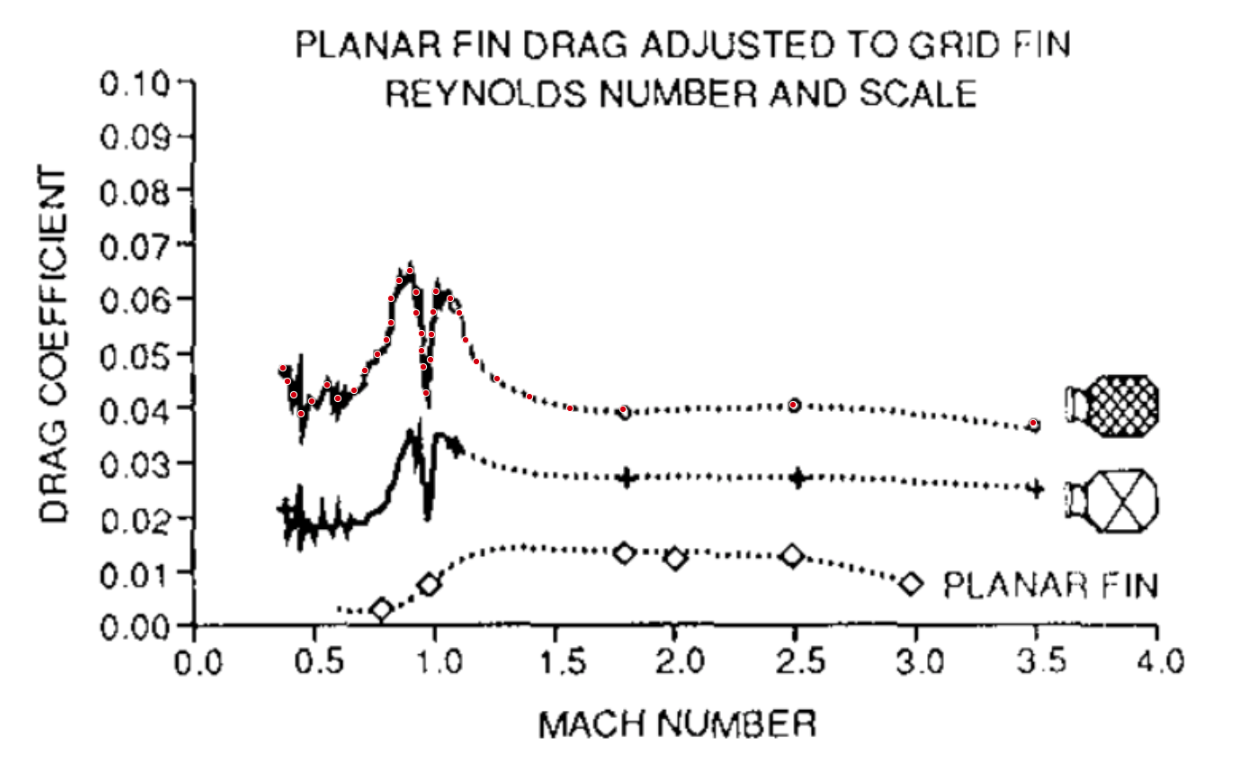
\includegraphics[width=\linewidth]{figures/LiteratureStudy/GridFins/DragCoefficientInterpolation.png}
        \caption{$C_D$ of a fin with points selected for interpolation \cite{washington1993grid}}
        \label{fig:drag_coeff_grid}
    \end{subfigure}
    \hfill
    \begin{subfigure}[b]{0.48\linewidth}
        \centering
        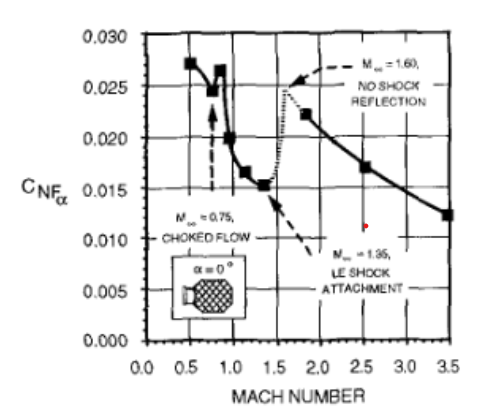
\includegraphics[width=\linewidth]{figures/LiteratureStudy/GridFins/CNGalpha_GF.png}
        \caption{$C_{N_\alpha}$ of a grid fin \cite{washington1993grid}}
        \label{fig:cnalpha_grid}
    \end{subfigure}
    \caption{Side-by-side comparison of drag coefficient and normal-force gradient for a grid fin}
    \label{fig:gridfin_side_by_side}
\end{figure}

The local angle of attack is the angle of the grid fin to the perpendicular direction of the flow. \autoref{eq:grid_fin_local_alpha} shows the local angle of attack for the left and right grid fins dependent on the effective angle of attack (descent angle of attack) and their respective deflection angles. The deflection angles go counter-clockwise, so an upward right grid fin deflection and a negative left grid fin deflection are positive.

\begin{equation}
\begin{aligned}
    \alpha_{l,R} =& \alpha_{eff} - \delta \\
    \alpha_{l,L} =& \alpha_{eff} + \delta 
\end{aligned}
\label{eq:grid_fin_local_alpha}
\end{equation}

With the angle of attack acting on each grid fin defined, the normal and axial force can be found from \autoref{fig:ACS_FBD}. First, the axial forces are the same for each grid fin as they are only dependent on Mach number. Second, the grid fins in the center of our 2D rocket are only modelled to give axial force as the third dimension is not considered.

\begin{equation}
\begin{aligned}
    F_a =& q \cdot S \cdot C_a(M) \\
    F_{N,L} =& q \cdot S \cdot C_n(M,\alpha_{l,L}) \\
    F_{N,R} =& q \cdot S \cdot C_n(M,\alpha_{l,R}) \\
\end{aligned}
\label{eq:grid_fin_aero_forces}
\end{equation}

The freebody diagram of the rocket during descent with grid fins is shown in \autoref{fig:ACS_FBD}. From this the perpendicular and parallel (x'', y'') forces are derived in \autoref{eq:ACS_para_perp}.

\begin{figure}[H]
    \centering
    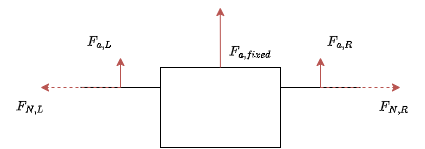
\includegraphics[width=0.5\linewidth]{figures/LiteratureStudy/GridFins/ACS_simple.png}
    \caption{Aerodynamic Control Surfaces freebody diagram during descent.}
    \label{fig:ACS_FBD}
\end{figure}

\begin{equation}
\begin{aligned}
    F_{x''} =& F_a \cdot (\cos(\delta_R) - \cos(\delta_L)) -F_{N,L} \cdot \cos(\delta_L) + F_{N_R} \cdot \cos(\delta_R) \\
    F_{y''} =& F_a \cdot (2 + \sin(\delta_L) + \sin(\delta_R)) - F_{N,L} \cdot \cos(\delta_L) + F_{N,R} \cdot \cos(\delta_R) \\
    M_z =& -(d_{gf}-d_{cg}) \cdot \bigg(F_a \cdot (\cos(\delta_R) - \cos(\delta_L)) -F_{N,L} \cdot \cos(\delta_L) + F_{N_R} \cdot \cos(\delta_R)\bigg) \\&+ r_r \cdot \bigg(F_{a} \cdot(\sin(\delta_R)-\sin(\delta_L) )+ F_{N,R} \cdot \cos(\delta_R) + F_{N,L} \cdot \cos(\delta_L)\bigg)
\end{aligned}
\label{eq:ACS_para_perp}
\end{equation}

